% Generated by ArticleSignalDiagrams. Opaque vector fills only.
\documentclass[10pt,tikz,border=5pt]{standalone}
\usepackage{lmodern}
\usetikzlibrary{fit}
\begin{document}
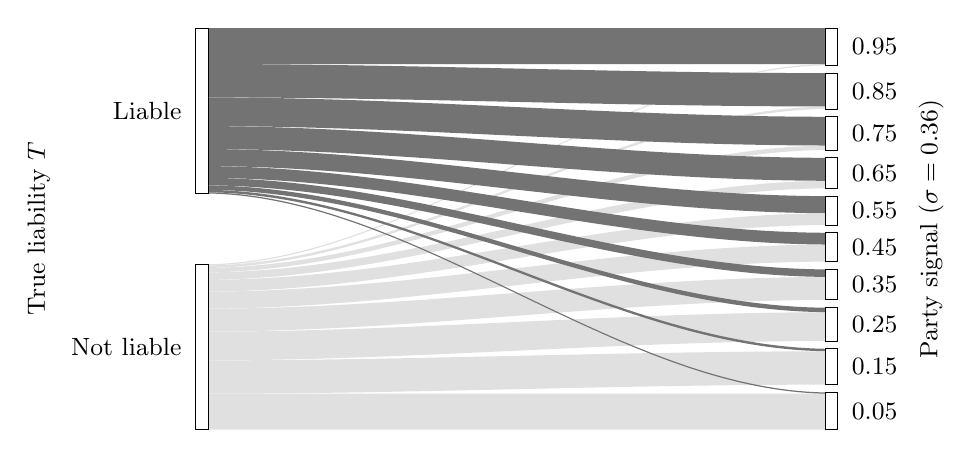
\begin{tikzpicture}[x=1cm,y=1cm,font=\small]\path[fill=black!12,draw=none] (3.3,-5.1) .. controls (6,-5.1) and (8.6,-5.1) .. (11.3,-5.1) -- (11.3,-4.643759) .. controls (8.6,-4.643759) and (6,-4.643759) .. (3.3,-4.643759) -- cycle;
\path[fill=black!12,draw=none] (3.3,-4.643759) .. controls (6,-4.643759) and (8.6,-4.527875) .. (11.3,-4.527875) -- (11.3,-4.104436) .. controls (8.6,-4.104436) and (6,-4.22032) .. (3.3,-4.22032) -- cycle;
\path[fill=black!12,draw=none] (3.3,-4.22032) .. controls (6,-4.22032) and (8.6,-3.973346) .. (11.3,-3.973346) -- (11.3,-3.608607) .. controls (8.6,-3.608607) and (6,-3.855581) .. (3.3,-3.855581) -- cycle;
\path[fill=black!12,draw=none] (3.3,-3.855581) .. controls (6,-3.855581) and (8.6,-3.45213) .. (11.3,-3.45213) -- (11.3,-3.160543) .. controls (8.6,-3.160543) and (6,-3.563994) .. (3.3,-3.563994) -- cycle;
\path[fill=black!12,draw=none] (3.3,-3.563994) .. controls (6,-3.563994) and (8.6,-2.965329) .. (11.3,-2.965329) -- (11.3,-2.748981) .. controls (8.6,-2.748981) and (6,-3.347646) .. (3.3,-3.347646) -- cycle;
\path[fill=black!12,draw=none] (3.3,-3.347646) .. controls (6,-3.347646) and (8.6,-2.5) .. (11.3,-2.5) -- (11.3,-2.351019) .. controls (8.6,-2.351019) and (6,-3.198665) .. (3.3,-3.198665) -- cycle;
\path[fill=black!12,draw=none] (3.3,-3.198665) .. controls (6,-3.198665) and (8.6,-2.034671) .. (11.3,-2.034671) -- (11.3,-1.939457) .. controls (8.6,-1.939457) and (6,-3.103451) .. (3.3,-3.103451) -- cycle;
\path[fill=black!12,draw=none] (3.3,-3.103451) .. controls (6,-3.103451) and (8.6,-1.54787) .. (11.3,-1.54787) -- (11.3,-1.491393) .. controls (8.6,-1.491393) and (6,-3.046974) .. (3.3,-3.046974) -- cycle;
\path[fill=black!12,draw=none] (3.3,-3.046974) .. controls (6,-3.046974) and (8.6,-1.026654) .. (11.3,-1.026654) -- (11.3,-0.995564) .. controls (8.6,-0.995564) and (6,-3.015884) .. (3.3,-3.015884) -- cycle;
\path[fill=black!12,draw=none] (3.3,-3.015884) .. controls (6,-3.015884) and (8.6,-0.472125) .. (11.3,-0.472125) -- (11.3,-0.456241) .. controls (8.6,-0.456241) and (6,-3) .. (3.3,-3) -- cycle;
\path[fill=black!55,draw=none] (3.3,-2.1) .. controls (6,-2.1) and (8.6,-4.643759) .. (11.3,-4.643759) -- (11.3,-4.627875) .. controls (8.6,-4.627875) and (6,-2.084116) .. (3.3,-2.084116) -- cycle;
\path[fill=black!55,draw=none] (3.3,-2.084116) .. controls (6,-2.084116) and (8.6,-4.104436) .. (11.3,-4.104436) -- (11.3,-4.073346) .. controls (8.6,-4.073346) and (6,-2.053026) .. (3.3,-2.053026) -- cycle;
\path[fill=black!55,draw=none] (3.3,-2.053026) .. controls (6,-2.053026) and (8.6,-3.608607) .. (11.3,-3.608607) -- (11.3,-3.55213) .. controls (8.6,-3.55213) and (6,-1.996549) .. (3.3,-1.996549) -- cycle;
\path[fill=black!55,draw=none] (3.3,-1.996549) .. controls (6,-1.996549) and (8.6,-3.160543) .. (11.3,-3.160543) -- (11.3,-3.065329) .. controls (8.6,-3.065329) and (6,-1.901335) .. (3.3,-1.901335) -- cycle;
\path[fill=black!55,draw=none] (3.3,-1.901335) .. controls (6,-1.901335) and (8.6,-2.748981) .. (11.3,-2.748981) -- (11.3,-2.6) .. controls (8.6,-2.6) and (6,-1.752354) .. (3.3,-1.752354) -- cycle;
\path[fill=black!55,draw=none] (3.3,-1.752354) .. controls (6,-1.752354) and (8.6,-2.351019) .. (11.3,-2.351019) -- (11.3,-2.134671) .. controls (8.6,-2.134671) and (6,-1.536006) .. (3.3,-1.536006) -- cycle;
\path[fill=black!55,draw=none] (3.3,-1.536006) .. controls (6,-1.536006) and (8.6,-1.939457) .. (11.3,-1.939457) -- (11.3,-1.64787) .. controls (8.6,-1.64787) and (6,-1.244419) .. (3.3,-1.244419) -- cycle;
\path[fill=black!55,draw=none] (3.3,-1.244419) .. controls (6,-1.244419) and (8.6,-1.491393) .. (11.3,-1.491393) -- (11.3,-1.126654) .. controls (8.6,-1.126654) and (6,-0.87968) .. (3.3,-0.87968) -- cycle;
\path[fill=black!55,draw=none] (3.3,-0.87968) .. controls (6,-0.87968) and (8.6,-0.995564) .. (11.3,-0.995564) -- (11.3,-0.572125) .. controls (8.6,-0.572125) and (6,-0.456241) .. (3.3,-0.456241) -- cycle;
\path[fill=black!55,draw=none] (3.3,-0.456241) .. controls (6,-0.456241) and (8.6,-0.456241) .. (11.3,-0.456241) -- (11.3,-0) .. controls (8.6,-0) and (6,-0) .. (3.3,-0) -- cycle;
\coordinate (axis-midline-0) at (0,-2.55);
\path[fill=white,draw=black,line width=0.3pt] (3.22,-5.1) rectangle (3.38,-3);
\node[anchor=east,fill=white,inner sep=2pt] (bucket-0-0-0) at (3.12,-4.05) {Not liable};
\path[fill=white,draw=black,line width=0.3pt] (3.22,-2.1) rectangle (3.38,-0);
\node[anchor=east,fill=white,inner sep=2pt] (bucket-0-0-1) at (3.12,-1.05) {Liable};
\node[fit=(bucket-0-0-0) (bucket-0-0-1),inner sep=0pt] (source-labels-0) {};
\coordinate (axis-title-0-0) at (source-labels-0.west |- axis-midline-0);
\node[rotate=90,anchor=south,inner sep=0pt] at ([xshift=-0.18cm]axis-title-0-0) {True liability $T$};
\path[fill=white,draw=black,line width=0.3pt] (11.22,-5.1) rectangle (11.38,-4.627875);
\node[anchor=west,fill=white,inner sep=2pt] (bucket-0-1-0) at (11.48,-4.863937) {0.05};
\path[fill=white,draw=black,line width=0.3pt] (11.22,-4.527875) rectangle (11.38,-4.073346);
\node[anchor=west,fill=white,inner sep=2pt] (bucket-0-1-1) at (11.48,-4.30061) {0.15};
\path[fill=white,draw=black,line width=0.3pt] (11.22,-3.973346) rectangle (11.38,-3.55213);
\node[anchor=west,fill=white,inner sep=2pt] (bucket-0-1-2) at (11.48,-3.762738) {0.25};
\path[fill=white,draw=black,line width=0.3pt] (11.22,-3.45213) rectangle (11.38,-3.065329);
\node[anchor=west,fill=white,inner sep=2pt] (bucket-0-1-3) at (11.48,-3.258729) {0.35};
\path[fill=white,draw=black,line width=0.3pt] (11.22,-2.965329) rectangle (11.38,-2.6);
\node[anchor=west,fill=white,inner sep=2pt] (bucket-0-1-4) at (11.48,-2.782664) {0.45};
\path[fill=white,draw=black,line width=0.3pt] (11.22,-2.5) rectangle (11.38,-2.134671);
\node[anchor=west,fill=white,inner sep=2pt] (bucket-0-1-5) at (11.48,-2.317336) {0.55};
\path[fill=white,draw=black,line width=0.3pt] (11.22,-2.034671) rectangle (11.38,-1.64787);
\node[anchor=west,fill=white,inner sep=2pt] (bucket-0-1-6) at (11.48,-1.841271) {0.65};
\path[fill=white,draw=black,line width=0.3pt] (11.22,-1.54787) rectangle (11.38,-1.126654);
\node[anchor=west,fill=white,inner sep=2pt] (bucket-0-1-7) at (11.48,-1.337262) {0.75};
\path[fill=white,draw=black,line width=0.3pt] (11.22,-1.026654) rectangle (11.38,-0.572125);
\node[anchor=west,fill=white,inner sep=2pt] (bucket-0-1-8) at (11.48,-0.79939) {0.85};
\path[fill=white,draw=black,line width=0.3pt] (11.22,-0.472125) rectangle (11.38,-0);
\node[anchor=west,fill=white,inner sep=2pt] (bucket-0-1-9) at (11.48,-0.236063) {0.95};
\node[fit=(bucket-0-1-0) (bucket-0-1-1) (bucket-0-1-2) (bucket-0-1-3) (bucket-0-1-4) (bucket-0-1-5) (bucket-0-1-6) (bucket-0-1-7) (bucket-0-1-8) (bucket-0-1-9),inner sep=0pt] (destination-labels-0) {};
\coordinate (axis-title-0-1) at (destination-labels-0.east |- axis-midline-0);
\node[rotate=90,anchor=north,inner sep=0pt] at ([xshift=0.18cm]axis-title-0-1) {Party signal ($\sigma=0.36$)};
\end{tikzpicture}
\end{document}

